\begin{table}[th]\Large
\centering
\caption{Performace of explanation generation. Our system outperforms MOCHEG on equivalent settings. Gold Evidence denotes ground truth text and image evidence while System Evidence means automatically retrieved text and image evidence. Gold Truthfulness denotes ground truth truthfulness label while System Truthfulness means the predicted truthfulness label.}
\resizebox{\textwidth}{!}{
\begin{tabular}{l|cccccc}
\hline
\textbf{Setting} & \textbf{ROUGE 1 (\%)} & \textbf{ROUGE 2 (\%)} & \textbf{ROUGE L (\%)} & \textbf{BLEU (\%)} & \textbf{BERTScore (\%)}\\ \hline
MOCHEG w/ Gold Evidence, Gold Truthfulness      & \textbf{45.5}   & \textbf{27.3}   & \textbf{35.4}   & \textbf{21.8}   & \textbf{89.0}   \\
MOCHEG w/ Gold Evidence, System Truthfulness    & 43.8   & 26.3   & 34.1   & 20.8   & 88.8   \\
MOCHEG w/ System Evidence, Gold Truthfulness    & 35.5   & 17.4   & \textbf{26.0}   & \textbf{10.9}   & 87.0   \\
MOCHEG w/ System Evidence, System Truthfulness  & 33.8   & 16.5   & 24.8   & 10.0   & 86.9   \\
Our w/ System Evidence, Gold Truthfulness      & \textbf{36.7}   & \textbf{17.9}   & 25.7   & 10.7   & \textbf{87.3}  \\
Our w/ System Evidence, System Truthfulness    & 34.3   & 16.8   & 25.4   & 10.4   & 87.1  \\\hline
\end{tabular}}
\label{label:explanation_generation}
\end{table}

In order to assess the degree to which our generated summaries contain the relevant facts necessary to fact-check the generated claims, we measure the ability of a method to generate an~\textit{explanation} of the predicted truthfulness label using our summary. We adopt a methodology similar to~\citet{Yao_2023}, where we consider the input claim $C$, its truthfulness label $Y_C$, and the summary for fact-checking $\{T_1, T_2, ...\}$ generated from~\textbf{MetaSumPerceiver}.  These components are concatenated into an overall sequence $X$ using a separator </s>. During the training of the rationale generator, We employ the actual truthfulness label of each claim as input. Critically, we do not retrain or fine-tune~\textbf{MetaSumPerceiver} for this task. In the evaluation phase, we utilize the truthfulness label predicted by the fixed entailment models. Following~\citet{Yao_2023}, we utilize BART based to generate the ruling statement. Our evaluation metrics include ROUGE~\cite{lin-2004-rouge}, BLEU~\cite{10.3115/1073083.1073135}, and Bertscore~\cite{zhang2020bertscore}. To assess the performance of explanation generation, we compare it with MOCHEG~\cite{Yao_2023}, as shown in Table~\ref{label:explanation_generation}.

\begin{figure*}[th]
  \centering
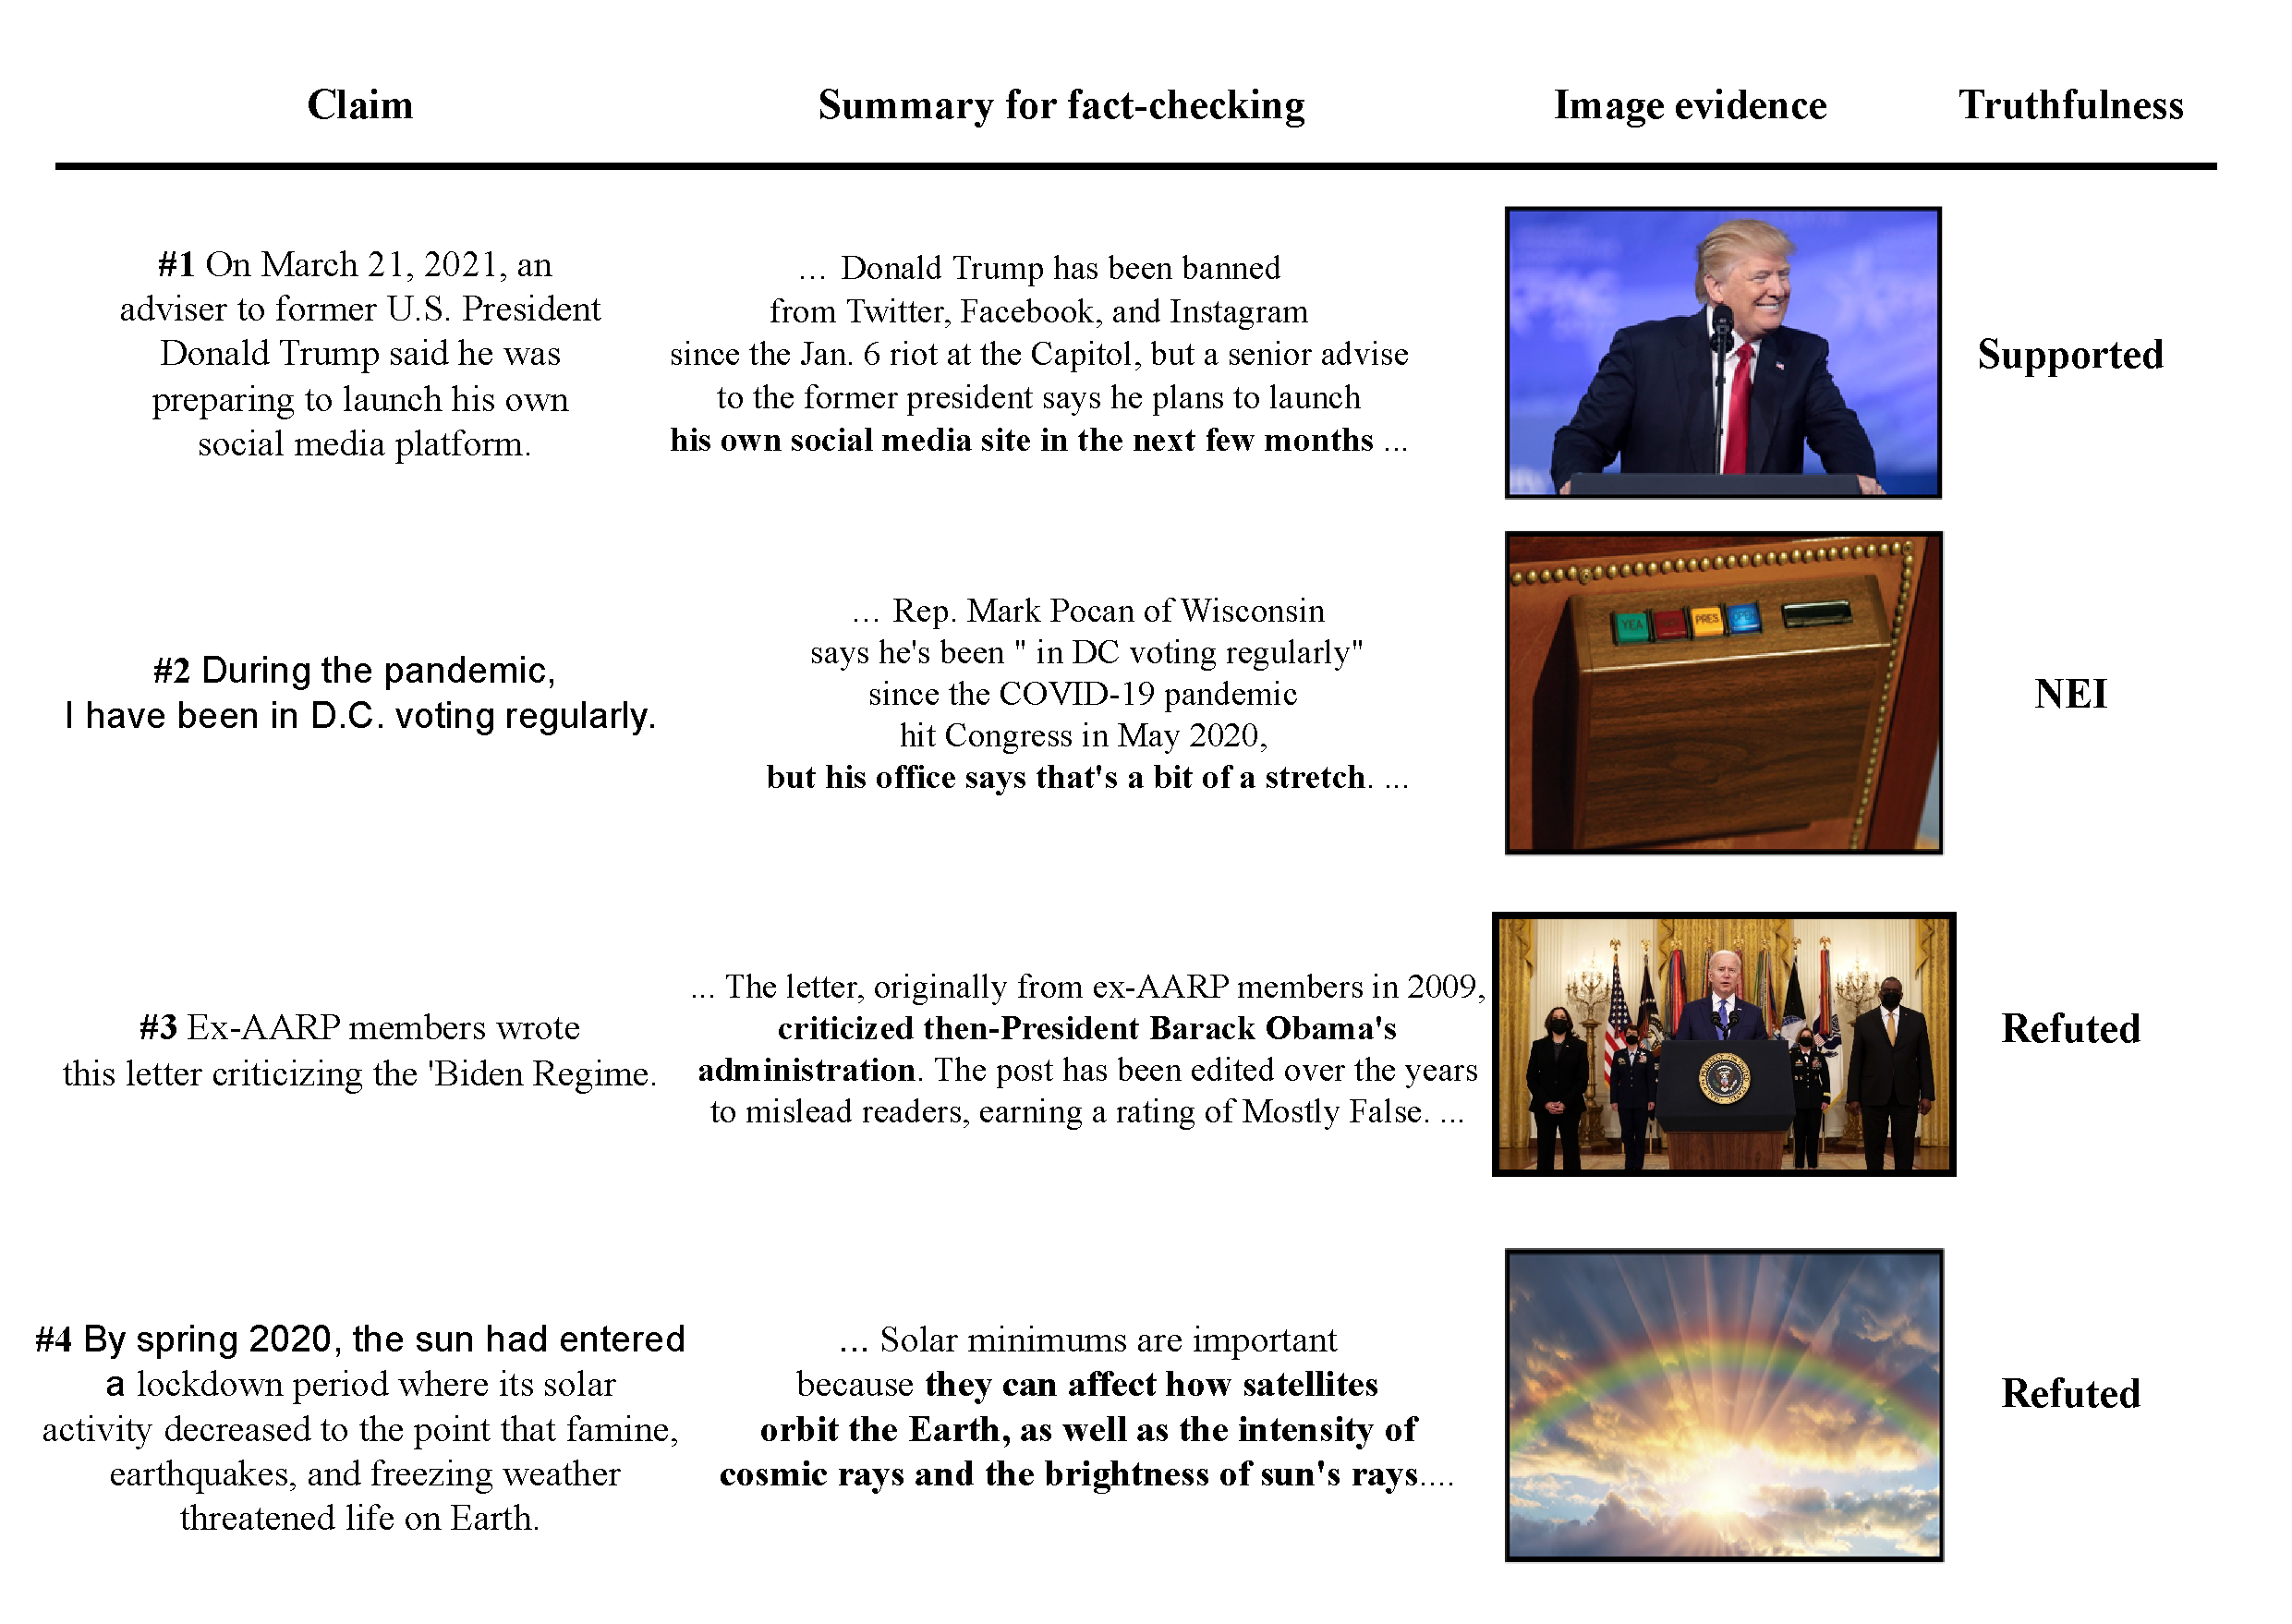
\includegraphics[width=\textwidth,height=\textwidth,keepaspectratio]{images/multimodal-fact-checking.pdf}
  \caption{Evidence summary examples in the explanation generation task. The truthfulness column shows gold labels. For instance, the third claim's article primarily discusses a letter critiquing the Obama administration. However, given President Joe's past collaboration with Ex-President Obama, the letter was manipulated to criticize the 'Biden Regime.' This assertion lacks support from credible sources, making it a refuted claim.}
  \label{fig:qualitative}
\end{figure*}

We observe that our model outperforms MOCHEG's evidence-retrieval-based method ("system evidence") on the rationale generation task. In our case, "system evidence" is our generated summary. We note that MOCHEG's method relies on retrieval from a pool of multimodal documents. The ground truth explanations rely on these sentences and thus may share some phrasing. This gives a slight advantage to MOCHEG's method on some metrics that measure n-gram overlap, whereas our method based on summarization may rephrase the same evidence. Nevertheless, we observe that our system outperforms MOCHEG's generated explanations. We further observe that our explanations generated using system evidence and system truthfulness outperform MOCHEG's method, which relies on the ground truth truthfulness label on the BERTScore metric. Overall, these results demonstrate that our summarizer, which was not trained for the rationale prediction task, is capturing relevant evidence across modalities in a short summary better than MOCHEG's evidence retrieval-based approach.

We illustrate our generated summaries for fact-checking in Figure~\ref{fig:qualitative}. Our results show that our summaries contain sufficient evidence to determine the accuracy of the claim label. Whether the truthfulness label is supported, labeled as NEI (No Evidence Identified), or refuted, we consistently provide evidence for a fact-checker to make a determination of the truthfulness of the claim.

\begin{table}[h]\Large
\centering
\caption{Evaluating the effectiveness of our multimodal multi-document claims using the pre-trained claim detection model.}
\begin{tabular}{l|c}
\hline
\textbf{Claim classes}                    & \textbf{Category percentage(\%)}  \\\hline
Unimportant Factual Sentence (UFS)        & 17.67          \\
Check-worthy Factual Sentence (CFS)       & 68.6           \\
Non-factual Sentence (NFS)                & 13.71          \\\hline
\end{tabular}
\label{label:claim_detect}
\end{table}
